% !TeX root = ../artigo.tex
\section{RESULTADOS E DISCUSSÃO}
Para testar o gerador de tráfego proposto, bastar realizar a criação de um script de simulação e utilizar as estruturas criadas e armazenadas no diretório \verb|/src/application/helper/| para facilitar a utilização do gerador de tráfego.

A Figura \ref{fig:script-simulação} apresenta um script simples para teste do gerador de tráfego. Nas linhas 34 e 35 dois nós são criados para assumirem o papel de cliente e servidor na simulação. Em seguida, nas linhas 38 e 39 uma instância da pilha de protocolos da Internet é criada e instalada nos dois nós da rede. Os dois nós são então conectados por um enlace ponto a ponto, com os parâmetros dessa conexão definidos nas linhas 42 a 46.

Em seguida, uma sub-rede é criada e o endereçamento IP dos nós da rede são estabelecidos e atribuídos (linhas 48 a 51). Com nós criados, conectados e com endereçamento adequado, precisamos instalar as aplicações. Isso ocorre nas linhas 58 a 62.

Com a topologia da simulação estabelecida, passa-se à definição do tempo de simulação. Serão 10 segundos (linha 70), considerando a realidade simulada. O tempo real pode variar bastante dependendo da complexidade da rede. Neste caso a simulação é simples e é executada quase que instantaneamente. É preciso ficar atento ao agendamento do início das aplicações. Repare que a aplicação do servidor é iniciada primeiro, com um segundo de simulação (linha 64). Já o cliente se inicia aos dois segundos de simulação. Dessa forma, quando o cliente for iniciado, o servidor já estará apto a receber as solicitações.

O último trecho do script apresenta estruturas para capturas de pacotes, e a execução da simulação propriamente dita.

\begin{figure}[!h]
	\centering
	\begin{subfigure}{\textwidth}
		\centering
		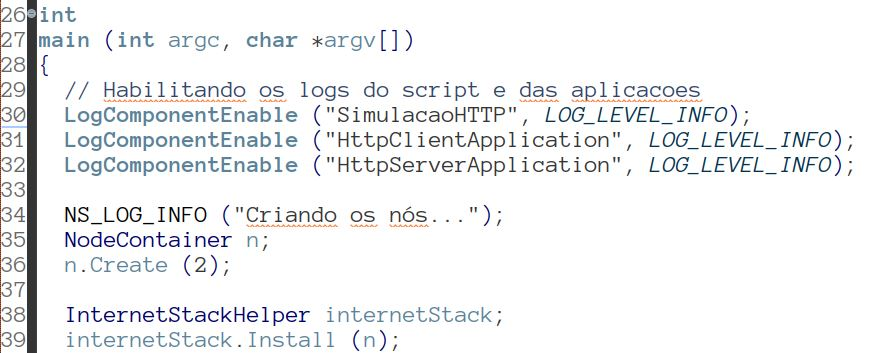
\includegraphics[width=0.7\linewidth]{textuais/script-simulação-1.jpg}
		\caption{}
		%\label{fig:sub1}
	\end{subfigure}
	\begin{subfigure}{\textwidth}
		\centering
		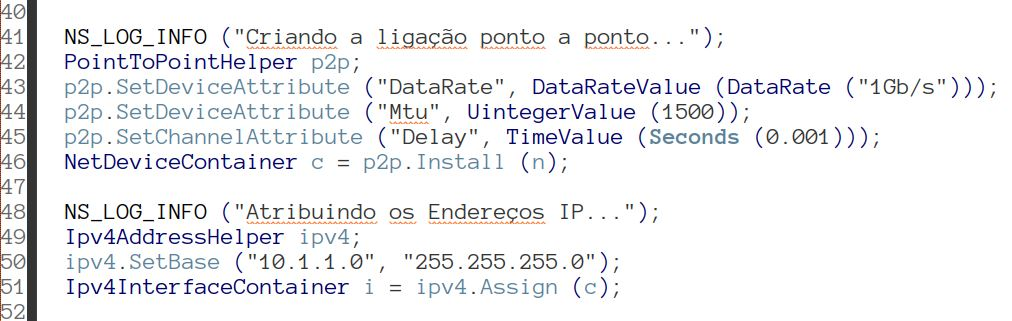
\includegraphics[width=0.7\linewidth]{textuais/script-simulação-2.jpg}
		\caption{}
		%\label{fig:sub2}
	\end{subfigure}
	\begin{subfigure}{\textwidth}
		\centering
		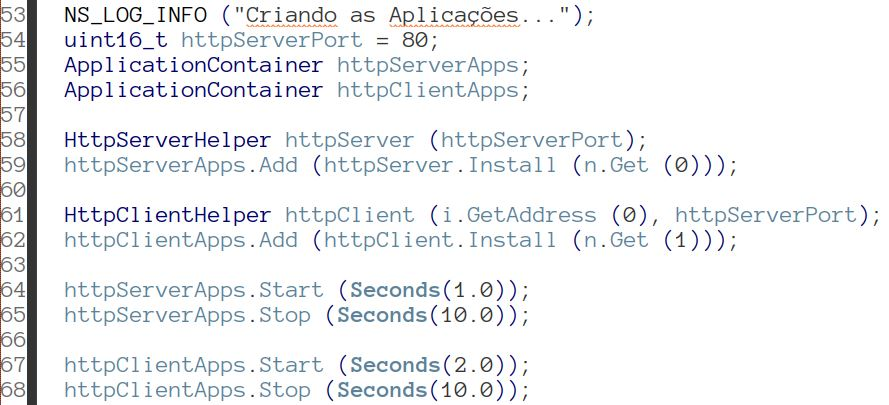
\includegraphics[width=0.7\linewidth]{textuais/script-simulação-3.jpg}
		\caption{}
		%\label{fig:sub2}
	\end{subfigure}
	\begin{subfigure}{\textwidth}
		\centering
		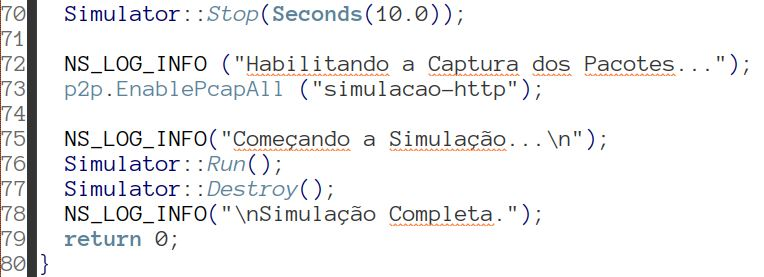
\includegraphics[width=0.7\linewidth]{textuais/script-simulação-4.jpg}
		\caption{}
		%\label{fig:sub2}
	\end{subfigure}
	\caption{Script de simulação para teste do gerador de tráfego.}
	\label{fig:script-simulação}
\end{figure}


Ao executar o script de simulação recebemos uma saída no console, com os principais acontecimentos da simulação, conforme apresentado na Figura \ref{fig:simulation-output}. O trecho da saída ilustrado mostra o passo a passo das trocas de mensagens entre os elementos do gerador de tráfego. O comportamento do gerador correspondeu ao esperado, com diferentes tamanhos de páginas e números de objetos \textit{inline}, de acordo com o modelo matemático estabelecido anteriormente.

\begin{figure}
	\centering
	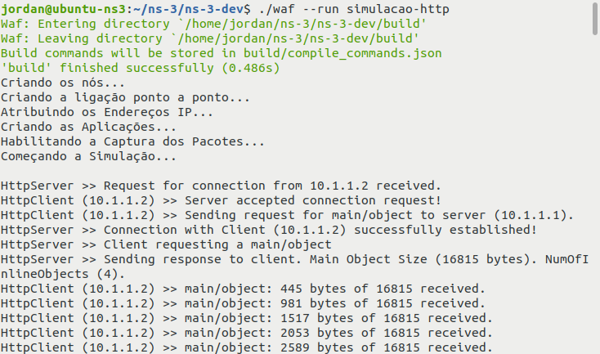
\includegraphics[scale=1]{textuais/simulation-output.png}
	\caption[Saída da execução do script de simulação.]{Saída da execução do script de simulação.
		\label{fig:simulation-output}}
\end{figure}

\subsection{Trabalhos Futuros}
Após a implementação bem-sucedida do modelo de tráfego web clássico de \cite{Pries2012}, foram inicializados estudos para a implementação de um modelo para transmissão de vídeo streaming, com base nos modelos citados por \cite{Navarro-Ortiz2020}. 

Durante essa fase do desenvolvimento, percebeu-se que para uma efetiva implementação desse modelo, seria necessário utilizar arquivos de vídeo no formato especial YUV, que por sua vez possibilitam a codificação (\textit{enconding}) de acordo com os parâmetros elencados em \cite{Navarro-Ortiz2020} e \cite{youtube-recommendations}. Esse pré -processamento é necessário para a posterior simulação da transmissão dos pacotes de streaming de vídeo a partir de módulos específicos para esta tarefa como o Evalvid \cite{evalvid}. Diante deste cenário, não houve tempo hábil para a implementação dessa etapa do projeto.

Outro tarefa futura é a revisão do código fonte e comentários para submissão do código para uma eventual inclusão na distribuição oficial do simulador ns-3.

